% Diese Zeile bitte -nicht- aendern.\pgfplotsset{compat=1.15}
\documentclass[course=erap]{aspdoc}
\graphicspath{ {./} }

%%%%%%%%%%%%%%%%%%%%%%%%%%%%%%%%%
%% TODO: Ersetzen Sie in den folgenden Zeilen die entsprechenden -Texte-
%% mit den richtigen Werten.
\newcommand{\theGroup}{140} % Beispiel: 42
\newcommand{\theNumber}{A208} % Beispiel: A123
\author{Tianhao Gu \and Zhongfang Wang \and Julien Escaig}
\date{Wintersemester 2023/24} % Beispiel: Wintersemester 2019/20
%%%%%%%%%%%%%%%%%%%%%%%%%%%%%%%%%

% Diese Zeile bitte -nicht- aendern.
\title{Gruppe \theGroup{} -- Abgabe zu Aufgabe \theNumber}

\begin{document}
\maketitle

\section{Einleitung}

\par
Das Ziel dieser Projektarbeit ist es, einen Algorithmus in C zu entwickeln, der ein farbiges Bild in ein Graustufenbild umwandelt und anschließend die Helligkeit des Graustufenbilds mithilfe der Gammakorrektur anpasst.

\par
Als Eingabe akzeptiert Unser Programm nur PPM-Dateien\cite{netpbm} des Typs P6. P6 bezieht sich dabei auf das Binärformat der Pixeldaten.  Diese besteht aus einem Header mit Metadaten, worauf die Pixel-Informationen folgen. Im Datenteil der PPM Datei gibt es für jeden Pixel genau drei Werte, die jeweils die Stärke der Farben Rot, Grün und Blau speichern. Je größer der Wert desto stärker ist die Farbe in einem bestimmten Pixel vertreten. Unterhalb ist ein einfaches Beispiel eines solchen Bildes.

\begin{figure}[h]
\begin{minipage}{0.45\textwidth}
\centering
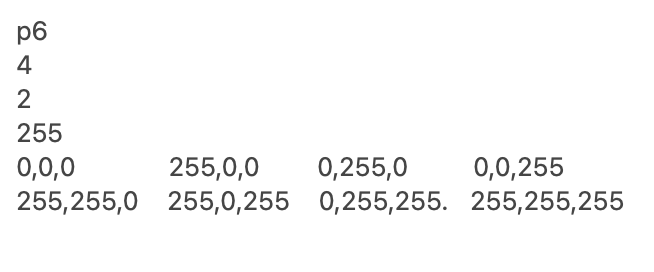
\includegraphics[width=\textwidth]{Bilder/demograph.png}
\caption{ein Beispiel für P6 PPM}
\end{minipage}
\hfill
\begin{minipage}{0.45\textwidth}
\centering

\includegraphics[width=\textwidth]{Bilder/demograph.ppm.png}
\caption{erzeugt durch den Beispielcode}
\end{minipage}
\end{figure}

\par
Die erste Phase des Projekts ist die Graustufenkodierung\cite{wikipedia2024grayscale}.Dafür verwenden wir die Formel (1) unten. Dabei wird der gewichtete Durchschnitt der Rot-, Grün- und Blau-Werte jedes Pixels ermittelt. Ein Beispiel ist in Abbildung 3 zu sehen. 
\begin{equation}
D(x,y)=\frac{a*R+b*G+c*B}{a+b+c}
\end{equation}


\begin{figure}[h]
\centering

\includegraphics[width=0.2\textwidth]{Bilder/gamma1.pgm.png}
\caption{Graustufen Konvertierung von Abbildung2}
\end{figure}

\par
Im zweiten Teil der Aufgabe befassen wir uns nun mit einem anderen Aspekt des menschlichen visuellen Systems (HVS) und zwar der Helligkeit\cite{wikipedia2023gammakorrektur}. Diese hat einen großen Einfluss darauf, wie natürlich ein Bild auf uns Menschen wirkt. Die Gammakorrektur ändert die Helligkeit bzw. den Kontrast eines Bildes, und hängt von der Wahl des $ \gamma $ Parameters ab.Bei diesem Algorithmus wird die Gammakorrektur durch folgende mathematische Formel (2) bestimmt. Die Werte D'(x,y) ergeben die Intensität der Graustufenkodierung für alle Pixel (x,y). Ein kleinerer Gammawert führt zu einem helleren Bild, während ein größerer Gammawert zu einem dunkleren Bild führt.

\begin{equation}
D'(x,y)={\left( \frac{D(x,y)}{255} \right)}^{\gamma}*255
\end{equation}

\par
Um den Effekt der Gammakorrektur zu visualisieren, betrachten wir nochmal die Abb.3. Unterhalb kann man 3 verschiedene „Helligkeits-Versionen“ von Abb.3 vergleichen.

\begin{figure}[h]
\begin{minipage}{0.3\textwidth}
\centering

\includegraphics[width=\textwidth]{Bilder/gamma0.1.pgm.png}
\caption{Gamma=0.1}
\end{minipage}
\hfill
\begin{minipage}{0.3\textwidth}
\centering

\includegraphics[width=\textwidth]{Bilder/gamma1.pgm.png}
\caption{Gamma=1}
\end{minipage}
\hfill
\begin{minipage}{0.3\textwidth}
\centering

\includegraphics[width=\textwidth]{Bilder/gamma10.pgm.png}
\caption{Gamma=10}
\end{minipage}
\end{figure}

\par
Die Hauptfunktion unsere Programms erhält 6 Parameter. Zwei davon sind \texttt{input\_file\_name} und \texttt{output\_file\_name}, welche die Pfade des Eingabebildes und des Ausgabebildes repräsentieren. Der Parameter \texttt{version} vom Datentyp \texttt{int} gibt die Version an. Der Parameter \texttt{benchmark\_number} repräsentiert die Anzahl der Benchmark-Zyklen. Die Parameter \texttt{a}, \texttt{b}, und \texttt{c} vom Datentyp \texttt{float} stellen die RGB-Gewichte für die Graustufenumwandlung dar. Schließlich erhält die Funktion noch einen Parameter \texttt{\_gamma} vom Datentyp \texttt{float}, der für den Gammawert steht.

\par
Obwohl die oben genannten Parameter zusätzlich zu den Ein- und Ausgängen standardmäßig mit sinnvollen Defaultwerten besetzt sind, kann der Nutzer diese Parameter auch selbst mit spezifischen und sinnvollen Werten ersetzen. Wenn die gesetzten Werte nicht sinnvoll sind, wird eine Fehlermeldung ausgegeben und das Programm wird beendet.Hier ist eine Übersicht an Optionen, die der Nutzer beim Aufrufen des Programms setzrn kann:

\begin{itemize}
\item Option \emph{-V<Zahl>} Die Option -V 0 ist die Standardimplementierung. -V 1 steht für die Implementierung V1 mit Taylorreihe. -V 2 steht für die Implementierung V2 mit SIMD. Andere Werte sind nicht erlaubt.
\item Option \emph{-B<Zahl>} Falls gesetzt, wird die Laufzeit der angegebenen Implementierung gemessen und ausgegeben. Das Argument gibt die Anzahl an Wiederholungen des Funktionsaufrufs an. Es darf nicht kleiner als 1000 sein.
\item Positionalem Argument \emph{<Dateiname>} Der Pfad zur Eingabedatei ist ein obligatorischer Parameter. Falls dieser ungültig ist, wird eine Fehlermeldung ausgegeben und das Programm wird beendet.
\item Option \emph{-o<Dateiname>} Der Pfad zur Ausgabedatei ist ein obligatorischer Parameter. Falls dieser ungültig ist, wird eine Fehlermeldung ausgegeben und das Programm wird beendet.
\item Option \emph{-{}-coeffs<FP Zahl>,<FP Zahl>,<FP Zahl>} Die drei Argumente müssen stets nicht-negativ sein und dürfen nicht den Wert Infinity und NaN annehmen. Ihre Summe darf auch nicht 0 betragen.
\item Option \emph{-{}-gamma<Floating Point Zahl>} Der Gammawert kann nicht negativ sein. Wenn diese Option nicht gesetzt wird, wird standardmäßig der Wert 1 verwendet.
\item Option \emph{-h|-{}-help} Eine Beschreibung aller Optionen des Programms und Verwendungsbeispiele werden ausgegeben und das Programm danach beendet. 
\end{itemize}

\section{Lösungsansatz}

\par
Es wird nun die Implementierung des Programms betrachtet. Zu Beginn erhält das Programm die Optionen und ihre Argumente von der Eingabe des Nutzers durch die Methode \texttt{getopt\_long}\cite{getoptlong3}. Nach erfolgreichem Einlesen der Eingabe wird die Funktion \texttt{check\_values} aufgerufen, um zu überprüfen, ob alle Argumente für das Programm legal sind. Bei illegalen Argumenten wird das Programm mit einer Fehlermeldung beendet.

\par
Die Versionsnummer der Implementierung kann entweder 0, 1 oder 2 sein. Bei den Versionen 0 und 1 werden lediglich sequenzielle Anweisungen verwendet. Version 2 wiederum verwendet SIMD-Instruktionen zur Berechnung der Graustufenkonvertierung.

\par
In allen aufgerufenen Funktionen wird zunächst die Eingabedatei gelesen. Gemäß der Netpbm-Dateibeschreibung ist die ppm-Datei in zwei Teile unterteilt: Metadaten und Pixelbereich. Es wird darauf geachtet, dass in den Metadaten ein Kommentar an beliebiger Stelle eingefügt werden kann. Daher wird beim Lesen der Metadaten in der ppm-Datei ein Zustandsautomat entworfen, um alle möglichen Randfälle abzufangen und zu behandeln. Die Automate wird gezeigt in Abbildung 7.

\begin{figure}[h]
\centering
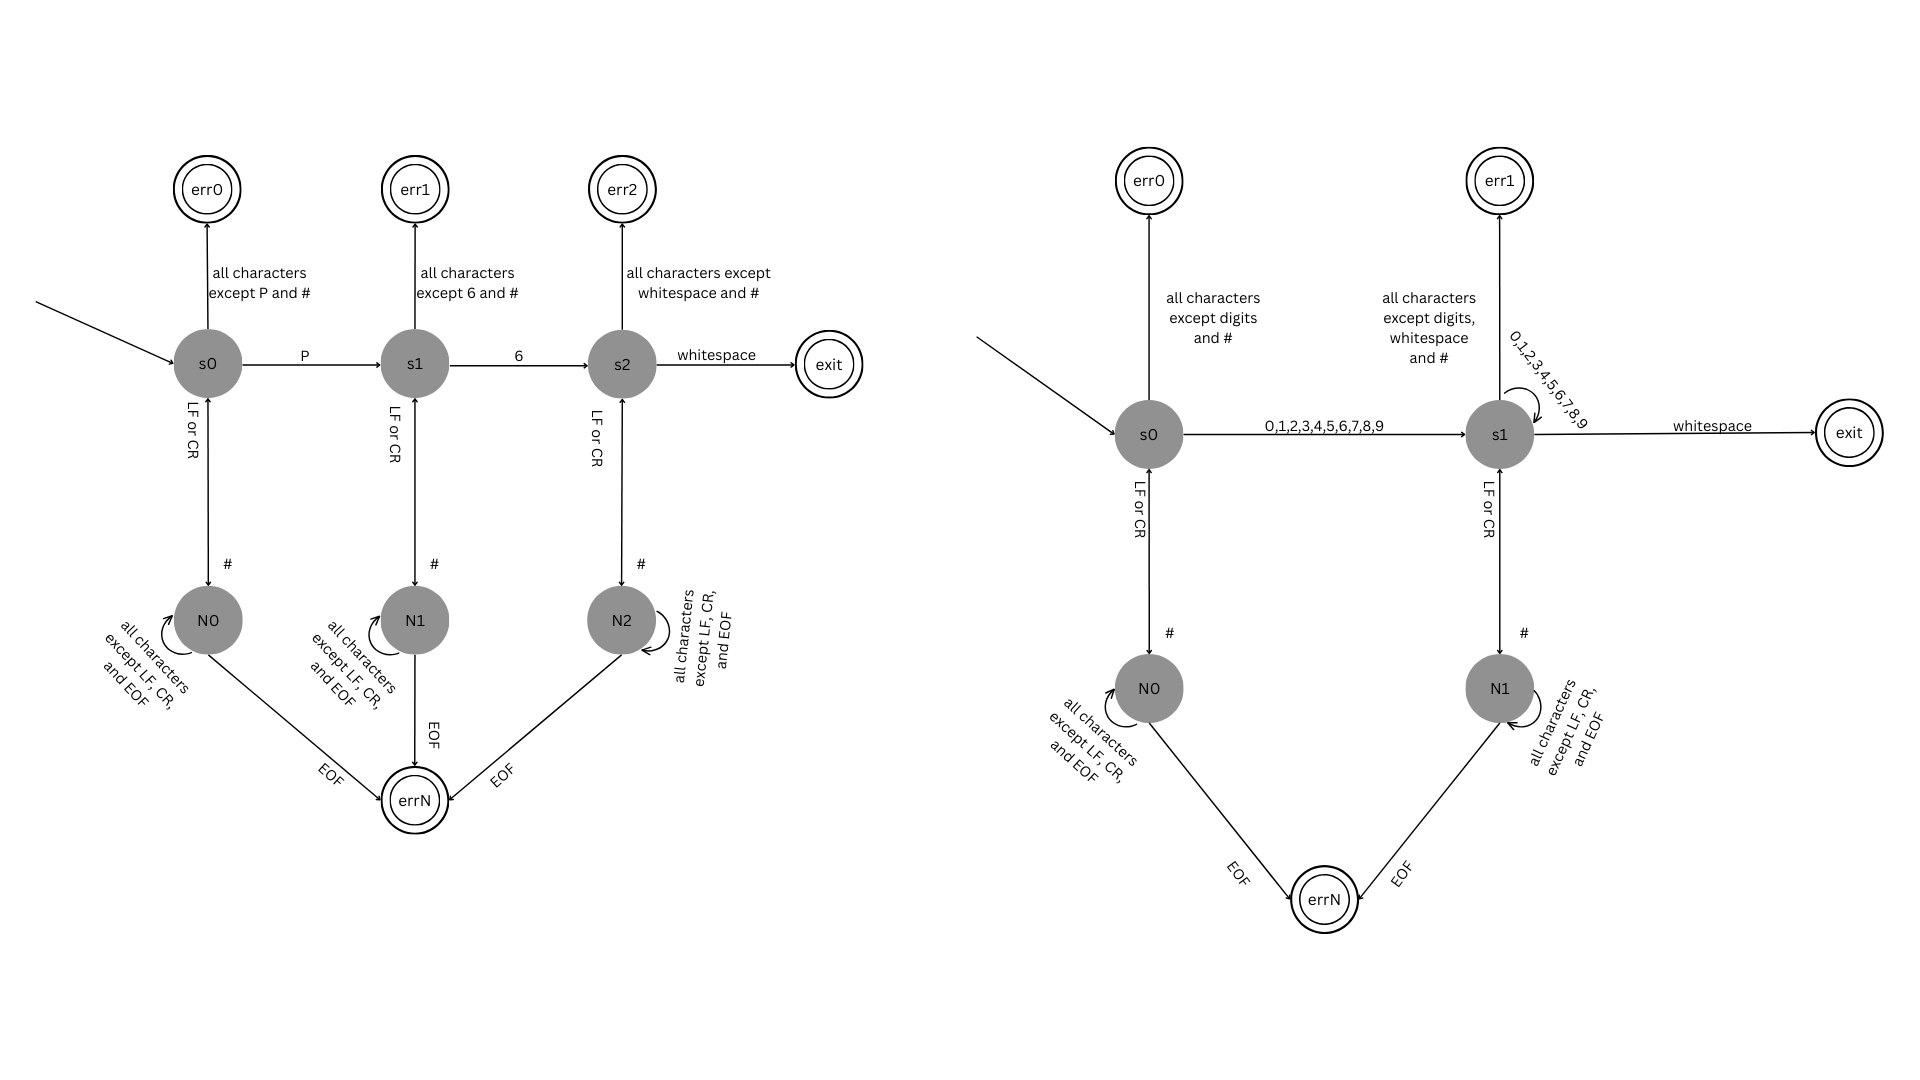
\includegraphics[width=1\textwidth]{Bilder/auto.png}
\caption{Zustandsautomat für das Lesen der Metadaten in der ppm-Datei}
\end{figure}

\par
Der Speicher für die Eingabedaten und Ausgabedaten wird basierend auf den Metadaten der Eingabedatei allokiert.Bei der Implementierung von V0 und V1 werden die drei Farben jedes Pixels beim Lesen der Eingabedatei in der originalen Reihenfolge gespeichert. Wenn V2 verwendet wird, werden beim Einlesen die drei Farben jedes Pixels getrennt gespeichert. Dadurch werden drei Speicherbereiche im Heap erstellt, die jeweils für eine bestimmte Farbe alle Pixel-Werte in fortlaufender Reihenfolge speichern. In der \texttt{main}-Funktion wird eine Switch-Anweisung verwendet, um verschiedene Funktionen gemäß der gewählten Versionen aufzurufen.

\par
In V2, der SIMD-Implementierung, wird \texttt{aligned\_alloc}\cite{man2022aligned_alloc} verwendet, um Speicher zu reservieren. Die Startadresse des Speichers wird auf ein Vielfaches von 16 ausgerichtet und erhöht damit die Geschwindigkeit des Ladens und Zurückschreibens von und aus dem Speicher in die xmm-Register. Anschließend wird die ausgewählte Version von gamma\_correct aufgerufen. In V0 und V1 wird die Graustufenkonvertierung für jeden Pixel sequentiell berechnet. V2 verwendet SIMD-Anweisungen, welche es ermöglichen die Graustufenwerte von vier Pixeln gleichzeitig zu berechnen. Hier noch eine Bemerkung: Wir setzen die Standardwerte von a, b, c wie folgt fest: a=0.299 b=0.587 c=0.114. Diese Gewichtungen werden häufig verwendet\cite{wikipedia2024grayscale}, weil sie in der Praxis gute Ergebnisse liefern und das menschliche Auge die Luminanzeigenschaften der Farben recht gut widerspiegeln. Nachdem die Graustufenwerte der Pixel berechnet wurden, verwenden V0 und V2 die \texttt{pow}-Funktion der \texttt{math.h} Bibliothek, um die Graustufenwerte nach der Gammakorrektur für jedes Pixel sequentiell zu berechnen. V1 verwendet keine Bibliotheksfunktionen.Als Nächstes sehen wir uns an, wie V1 grundlegende mathematische Verfahren zur Umsetzung von pow Funktion durch die Taylor-Entwicklung.

\par
Die Taylor Entwicklung\cite{mathworld2024taylorseries} ist eine lokale Approximation eines Funktionswertes der Form $f(x) = f(a) + f'(a)(x-a) + \frac{{f''(a)(x-a)^2}}{2!} + \frac{{f'''(a)(x-a)^3}}{3!} + \ldots + \frac{{f^n(a)(x-a)^n}}{n!} + R_n(x) $ Wir verwenden den Fall $a=1$ und erhalten die folgende Formel:

\begin{equation}
f(x) = 1 + \frac{(x-1)^1}{1!} (\gamma) + \frac{(x-1)^2}{2!} (\gamma)(\gamma-1)  + \cdots + \frac{(x-1)^n}{n!} \prod_{i=0}^{n-1} (\gamma-i) + R_n(x)
\end{equation}

\par
Betrachten wir zunächst die drei Grenzfälle:
\begin{enumerate}
\item Wenn die Basis kleiner oder gleich \(0.5\) ist und Gamma größer oder gleich \(150\) ist, ist das Ergebnis immer \(0\) (\textbf{Underflow} für \texttt{float}).
\item Wenn die Basis \(1.0\) beträgt, ist das Ergebnis immer \(1\).
\item Wenn Gamma größer ist als die magische Zahl \(67075968\), ist das Ergebnis \(0\), wenn die Basis kleiner als \(1\) ist (wieder \textbf{Underflow}).
\end{enumerate}

\par
Eine Beobachtung für Formel (2) ist, dass der Base \(D(x,y)/255\) immer eine Zahl zwischen 0 und 1 ist. \emph{Gamma} ist auf die Bedingung beschränkt, dass es größer als 0 und nicht \emph{Infinity} oder \emph{NaN} ist. Bei der Entwicklung haben wir festgestellt, dass die Berechnung von \(\prod_{i=0}^{n-1} (\gamma-i)\) bei größeren Gammawerten leicht zu einem \textbf{Overflow} führt. Um das Problem zu lösen, zerlegt V2 \emph{Gamma} in eine ganze Zahl und eine Dezimalzahl und berechnet diese separat.

\par
Für Den Ganzzahlanteil ist unser Design Gedanke, den Exponenten in eine binäre Zahl umzuwandeln und dann zu zerlegen. Im folgenden Beispiel wird die 29. Potenz von 0,79 berechnet

\[
29 = 1 \cdot 2^0 + 0 \cdot 2^1 + 1 \cdot 2^2 + 1 \cdot 2^3 + 1 \cdot 2^4
\]
\[
0.79^{29} = 0.79^{2^0} \cdot 0.79^{2^2} \cdot 0.79^{2^3} \cdot 0.79^{2^4}
\]

\par
Da Gamma kleiner als 67075968, also zwischen $2^{25}$ und $2^{26}$, so dass wir unabhängig vom Exponenten höchstens 26 Schleifen benötigen.

\par
Danach verwenden wir Formel (3) für den Bruchteil, und die Akkumulation endet, wenn der Expansionsterm klein genug ist. Hier ist zu beachten, dass wir das Ergebnis des i-ten Expansionsterms zur Berechnung des (i+1)-ten Expansionsterms verwenden können.

\par
Die Graustufenwerte nach der Gammakorrektur werden über einen weiteren Funktionsaufruf im Format von PGM in die Ausgabedatei geschrieben. PGM (Portable Gray Map) Format\cite{netpbm} wird zur Speicherung von Graustufenbildern verwendet, weil es ein einfaches, leicht umsetzbares Bildformat ist. Im Vergleich zu anderen komplexen Bilddateiformaten ist das PGM-Format sehr einfach. Es speichert die Pixelwerte des Bildes und kann leicht in Textform bearbeitet und gelesen werden. Dieses Format erfordert keine komplizierten Dekodierer oder zusätzliche Datenkompression, was es ideal für die schnelle Speicherung und Verarbeitung von Graustufenbilddaten macht. Bevor alle Ressourcen freigegeben werden, wird \texttt{gamma\_correct()} wiederholt ausgeführt, wenn der Benutzer die Option \texttt{-B} in den Optionen aktiviert hat. Die Zeit wird zu Beginn und am Ende des Zyklus aufgezeichnet. Diese Laufzeit des Zyklus wird später für die Leistungsanalyse verwendet.

\par
Am Ende des Programms müssen alle Ressourcen freigegeben werden. Zusätzlich wird an sämtlichen Stellen im Programm, an denen eine Allocation oder eine IO-Operation durchgeführt wird, überprüft, ob sie erfolgreich war.

\par
Das Programm verteilt alle Funktionen sinnvoll auf die verschiedenen Funktionen. Jede Funktion ist angemessen groß, logisch korrekt, leicht zu warten und vermeidet Blob Muster.

\section{Genauigkeit}

\par
Schauen wir uns die Ungenauigkeit an, die entstanden wäre, wenn das Programm in Version 2 anstelle von pow in stadard lib die Formel (3) verwendet hätte. Dies liegt daran, dass wir lediglich eine beschränkte Anzahl von Termen der Taylorreihe berechnen können. Dadurch werden Terme ab dem (n+1)-ten vernachlässigt, was zu Genauigkeitsverlusten führt. Zur Schätzung der Präzision ziehen wir das \text{Peano'sche Restglied}\cite{mathematiknet2009taylorpolynome} heran.

\[
o\left((x-1)^n\right)
\]

\par
Es zeigt sich, dass das Restglied bei einem Wert von x nahe null langsam und bei x nahe eins schneller konvergiert. Eine präzisere Beschreibung ermöglicht das Lagrange'sche Restglied\cite{biancahoegel2021taylorformel}, insbesondere da der Exponent ein Bruchteil des Gammas ist und wir uns auf Werte zwischen 0 und 1 konzentrieren. Wir setzen einen Anpassungspunkt von 1 ein und vereinfachen die Lagrangesche Gleichung wie folgt:

\[
\frac{{\prod_{i=0}^{n} (\gamma - i) \cdot (x-1)^{n+1}}}{{(n+1)!}} \label{eq:gamma_product}
\]

\par
Wir werden dies im Folgenden unter zwei Gesichtspunkten analysieren: Zum einen soll untersucht werden, wie viele Konvergenzterme erforderlich sind, um sich dem minimalen Wert von float zu nähern, und zum anderen soll untersucht werden, welche Kombinationen von Gamma und x zu Fehlern führen, die größer als 1/255 und welche kleiner als 1/255 sind. Der Fehler des endgültigen gamma-korrigierten Ergebnisses beträgt höchstens 1, wenn der Fehler weniger als 1/255 beträgt.

\par
Beginnen wir mit der ersten Perspektive, bei der wir gamma bzw. x fixieren und die Auswirkungen einer Änderung einer anderen Variablen auf die Anzahl der Iterationen untersuchen. Die Schlussfolgerung ist unten dargestellt.

\par
Daraus folgt, dass die Auswirkung von Gamma linear und die von der Basis krummlinig ist. Wenn also die Basis nahe null liegt, konvergiert sie langsam, was ebenfalls zu größeren Ungenauigkeiten führt.

\par
todo by tianhao

\par
Anschließend wird die Auswirkung der Änderung von (Gamma,x) auf den Fehler weiter untersucht. Hier verwenden wir den Referenzstandard netpbm/v0

\par
todo by zhongfang

\par
Aber wirkt sich das sehr negativ auf unsere Ergebnisse aus?In Anwendungen tatsächlich nicht wirklich schlimm.Begründen ist wie folgt:
\begin{enumerate}
\item Die Wahrscheinlichkeit ist sehr gering, wenn die Basis kleiner als 0,0001 ist.
\item Wenn die Basis klein und gleichzeitig Gamma groß ist, wird dies bereits als Grenzfall berücksichtigt.
\item Wenn das Gamma einen ganzzahligen Teil enthält, ist das Ergebnis des ganzzahligen Teils kleiner als 1, weil die Basis kleiner als 1 ist. Der absolute Fehler aus dem gebrochenen Teil der Berechnung wird reduziert, wenn wir das Ergebnis mit dem ganzzahligen Teil multiplizieren.
\end{enumerate}

\section{Performanzanalyse}

\par
todo by Julien


\section{Zusammenfassung und Ausblick}

\par
Bei diesem Projekt ging es darum, eine Graustufen-Kodierung und Gammakorrektur selber zu programmieren. Das Umsetzen der Graustufen-Kodierung war relativ einfach, genau wie die Implementierung mit der Pow-Funktion. Die Aufgabe erhielt eine neue Stufe an Komplexität, sobald es zur Implementierung mit der Taylorreihe und der SIMD Implementierung kommt. Die Taylorreihe führt zu einer geringeren Genauigkeit. Die SIMD-Funktion hat zu einer höhere Performanz von etwa … Prozent geführt. Abschließend kann man sagen, dass dieses Projekt einen interessanten Einblick in verschiedene Bildformate, das Approximieren mit Hilfe der Taylorreihe und das Optimieren mit Hilfe von SIMD-Intrinsics geliefert hat.

\par
Außerdem erörterten die Diskussionsteilnehmer, wie das Problem der langsamen Iteration gelöst werden kann, wenn x klein ist; eine Lösung ist die Verwendung von Lookup Table\cite{wikipedia2023lookuptable}.

\par
todo by zhongfang: explain how to use lookup table to solve the problem of slow convergence when x is small

% TODO: Fuegen Sie Ihre Quellen der Datei Ausarbeitung.bib hinzu
% Referenzieren Sie diese dann mit \cite{}.
% Beispiel: CR2 ist ein Register der x86-Architektur~\cite{intel2017man}.
\bibliographystyle{plain}
\bibliography{Ausarbeitung}

\end{document}



